\documentclass{article}
\usepackage{amsmath}
\usepackage{amsfonts}
\usepackage{amssymb}
\usepackage{amsthm}
\usepackage{geometry}
\usepackage{algorithm}
\usepackage{algpseudocode}
\usepackage{minted}
\usepackage{graphicx}
\usemintedstyle{xcode} % You can change this to 'monokai', 'github', 'xcode', etc.

\geometry{a4paper, left=2cm, right=2cm, top=2cm, bottom=2cm}

\title{Report for AI Capstone Homework 1: BEV Projection}
\author{FU, YONG-WEI (112550107) }
\date{\today}

\begin{document}

\maketitle

\section{Implementation}
\subsection{Code}
My implementation can be split into 6 main sections:

\subsubsection{Parameters Preparation}
\begin{minted}[linenos, breaklines, frame=lines, fontsize=\footnotesize]{python}
# 1. hardcode two camera positions and orientations in the world space
cam_bev = [0.0, 2.5, 0.0]
cam_front = [0.0, 1.0, 0.0]

pitch = -np.pi/2
yaw   = 0  
roll  = 0

# calculate parameters
center_x = self.width / 2
center_y = self.height / 2
fov_rad = fov / 180 * np.pi
f = (self.width / 2) / np.tan(fov_rad / 2) # similar triangles, knowing that tan = width/2 / focal_length

new_pixels = []
\end{minted}

First, I prepared the parameters of the cameras, both intrinsic and extrinsic ones. 
I recorded the position, difference between the BEV camera's orientation and the world coordinate system, and focal length of the cameras, as well as the center of the 
optical sensor (the pinhole). The focal length is derived using the image width and the given Field 
of View (FOV) via trigonometry:
\[
    \because\ \tan(\frac{\text{FOV}}{2}) = \frac{\frac{\text{width}}{2}}{f}
\]

\[
    \therefore\ f = \frac{\frac{\text{width}}{2}}{\tan(\frac{\text{FOV}}{2})}
\]

Lastly, I created an empty list to for the front camera to store the new pixel coordinates.

\subsubsection{Vector from sensor to pinhole}
\begin{minted}[linenos, breaklines, frame=lines, fontsize=\footnotesize]{python}
# 2. project the points to the floor 
for p in self.points:
    # first, we assume that the camera is looking horizontally
    # then this is a 3d vector starting from the pixel on the sensor plane and pointing towards the lens center
    from_pixel_to_pinhole_x = center_x - p[0]
    from_pixel_to_pinhole_y = center_y - p[1]
    from_pixel_to_pinhole_z = -f
\end{minted}
Then, I calculated the vector from the specified pixel to the pinhole in the BEV 
camera. This is simply done with subtracting the pixel coordinates from the coordinate of the pinhole.

\subsubsection{Vector rotation}
\begin{minted}[linenos, breaklines, frame=lines, fontsize=\footnotesize]{python}
    # Rotate ray to World Space using ONLY the BEV camera's absolute orientation 
    # 1. Pitch (X-axis)
    x1 = from_pixel_to_pinhole_x
    y1 = from_pixel_to_pinhole_y * np.cos(pitch) - from_pixel_to_pinhole_z * np.sin(pitch)
    z1 = from_pixel_to_pinhole_y * np.sin(pitch) + from_pixel_to_pinhole_z * np.cos(pitch)

    # 2. Yaw (Y-axis)
    x2 = x1 * np.cos(yaw) + z1 * np.sin(yaw)
    y2 = y1
    z2 = -x1 * np.sin(yaw) + z1 * np.cos(yaw)

    # 3. Roll (Z-axis)
    rot_x = x2 * np.cos(roll) - y2 * np.sin(roll)
    rot_y = x2 * np.sin(roll) + y2 * np.cos(roll)
    rot_z = z2
\end{minted}
But the concern here is that, that vector is living in the BEV camera's local coordinate system, 
not the world coordinate system, and these two are not the same. 
Therefore, we need to rotate it to the world coordinate system, in order to project it to the 
floor of the environment. This is done by rotating the vector with x, y, z axes in order, using 
the pitch, yaw, and roll angles we prepared in the first section. By this, we can get the true 
direction of the ray from the pixel to the pinhole, in the perspective of the world.

\subsubsection{Obtaining the world coordinates}
\begin{minted}[linenos, breaklines, frame=lines, fontsize=\footnotesize]{python}
    # find the intersection of the ray with the floor plane (y=0)
    t = cam_bev[1] / -rot_y
    
    # If t is negative, the ray is shooting backwards up into the sky
    if t < 0:
        continue
    
    # got t, scale all of them to find the absolute world coordinates on the floor
    floor_x = cam_bev[0] + rot_x * t
    floor_y = 0.0
    floor_z = cam_bev[2] + rot_z * t
\end{minted}
After getting the real direction of the ray, we can extend the ray so that it touches 
the floor (the plane with y=0). By this, we can get the world coordinates of the point on 
the floor that the user is originally clicking on in the view of the BEV camera.

\subsubsection{Projection onto the front camera}
\begin{minted}[linenos, breaklines, frame=lines, fontsize=\footnotesize]{python}
    # project them to the front camera
    # get the vector from the floor to the front camera pinhole
    from_floor_to_pinhole_x = cam_front[0] - floor_x
    from_floor_to_pinhole_y = cam_front[1] - floor_y
    from_floor_to_pinhole_z = cam_front[2] - floor_z
\end{minted}
Then, we can get the direction of the ray from the point on the floor to the optical center 
of the front camera. This is done by simply subtracting the world coordinates of the point 
on the floor from the position of the front camera.

\subsubsection{Calculating the new coordinates in the front camera}
\begin{minted}[linenos, breaklines, frame=lines, fontsize=\footnotesize]{python}
    # scale down to the focal length (similar triangles)
    # The signs naturally resolve because of the vector direction
    front_cam_x = from_floor_to_pinhole_x * f / from_floor_to_pinhole_z
    front_cam_y = from_floor_to_pinhole_y * f / from_floor_to_pinhole_z 
    
    # calculate the final pixel coordinates on the front image
    u_front = center_x + front_cam_x
    v_front = center_y + front_cam_y
    
    # record them
    new_pixels.append([int(u_front), int(v_front)])
\end{minted}
Lastly, after getting the direction of the ray, we can draw a vector from the pinhole of the 
front camera to the sensor plane using the same direction, and calculate the ending point of 
that vector on the sensor: that would be the new pixel coordinates in the front camera.
\\
Thus, we have completed the projection of the pixels from the BEV camera to the front camera.

\subsection{Result and Discussion}
\subsubsection{Results}
\begin{figure}[htbp]
    \centering
    \begin{minipage}{0.45\textwidth}
        \centering
        
\includegraphics[width=\textwidth]{images/bev1.png}
        \caption{BEV Camera of the 1st floor}
    \end{minipage}\hfill
    \begin{minipage}{0.45\textwidth}
        \centering
        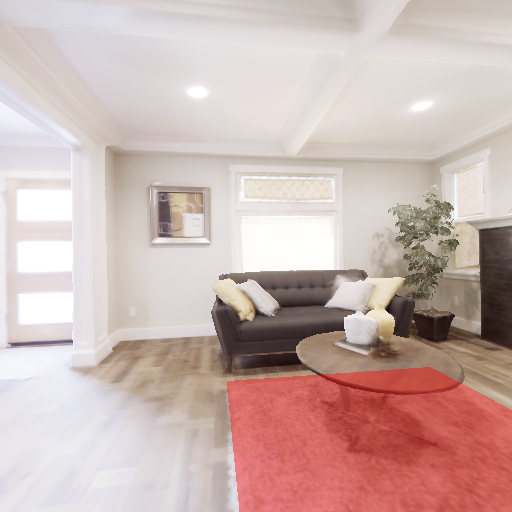
\includegraphics[width=\textwidth]{images/projection1.png}
        \caption{Front Camera Projection of the 1st floor}
    \end{minipage}
\end{figure}
\begin{figure}[htbp]
    \centering
    \begin{minipage}{0.45\textwidth}
        \centering
        
\includegraphics[width=\textwidth]{images/bev2.png}
        \caption{BEV Camera of the 2nd floor}
    \end{minipage}\hfill
    \begin{minipage}{0.45\textwidth}
        \centering
        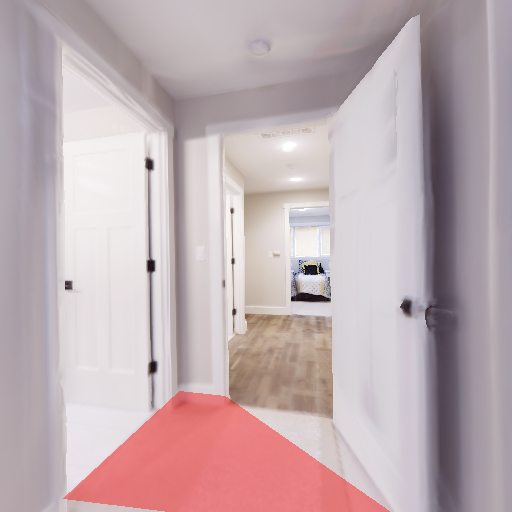
\includegraphics[width=\textwidth]{images/projection2.png}
        \caption{Front Camera Projection of the 2nd floor}
    \end{minipage}
\end{figure}

\subsubsection{Discussion}
In the implementation, i found a quite interesting property.
Back in middle school, we have learned that the projection of a pinhole camera would be 
inverted, meaning that the image on the sensor should be upside down and left-right reversed. For the 
human to see the correct image, the camera system must invert them back. And when tackling the coordinate tasks
like this one, if we don't invert them back at first, the result should be wrong. However, in this case, since we are doing two 
projections effectively (one from the BEV camera to the world, and one from the world to the front camera), 
the two inversions cancel each other out. Therefore, we can just simply ignore this inversion effect 
in the code, and the result would still be correct.

\subsubsection{References}
I mostly crafted the methods using my own knowledge and with the assistance of gemini. The
code is put into use only after i understood the mathematical and physical meaning behind each step. 

\section{Questions}
\subsection{(a) How do the intrinsic and extrinsic matrices contribute to the BEV-to-front-view projection?}
According to the definition, matrices are mathematical tools that represent linear transformations from one 
vector to another, and so are the intrinsic and extrinsic matrices here. In the context of camera projection, 
the intrinsic and extrinsic matrices serve as the bridges between different coordinate systems: the 3D world space, 
the 3D camera space, and the 2D pixel space.

\subsubsection{The Intrinsic Matrix:}
The intrinsic matrix contains the internal hardware parameters of the camera, primarily the focal length ($f$) 
and the optical center. It is responsible for the transformation between 2D pixels and 3D local camera coordinates.
In this assignment, the intrinsic matrix is used in these two situations:
\begin{itemize}
    \item \textbf{BEV Unprojection:} We utilize the inverse of the intrinsic matrix to transform the 2D pixel from the BEV image into a 3D ray starting from the camera sensor and pointing towards the pinhole.
    \item \textbf{Front Projection:} Once the final 3D point relative to the Front camera is calculated, the intrinsic matrix is used to squash that 3D point back down onto the sensor screen, giving us the final 2D pixel coordinates in the Front camera's image.
\end{itemize}

\subsubsection{The Extrinsic Matrix:} 
The extrinsic matrix contains the external parameters of the camera, and thus defines its position. 
It is responsible for the transformation between the camera's local 3D space and the global world space.
It's mainly used in these two situations in the assignment:
\begin{itemize}
    \item \textbf{BEV camera to world:} The BEV camera's extrinsic parameters rotate its local ray (Pitch, Yaw, Roll) and translate it to its physical height, forcing the ray 
    to be aligned with the world coordinate system and allowing it to intersect with the floor plane, giving us the world coordinates of that point on the floor.
    \item \textbf{World to Front camera:} The Front camera's extrinsic parameters are then used to calculate the vector from that world floor coordinate back to the 
    Front camera's local physical position, preparing it for the final 2D pixel projection.
\end{itemize}

\subsection{(b) What factors may cause projection misalignment? List at least two factors and explain the reason.}
Although this assignment can be solved with a simple procedure, real world scenarios remains complex and challenging. 
There are several factors that can make the projection in real life misalign or even fail, for instance:
\begin{itemize}
    \item \textbf{Lens Distortion:} In this ideal environment, we assume that the cameras are perfect pinhole cameras, but in reality, lenses 
    are usually not perfect pinholes (most of the times, convex lenses are used), and they can cause distortion on the edges or out of focus images, 
    introducing noise and errors into the projection process.
    \item \textbf{Mounting Errors:} The camera is ideally fixed at a certain position and orientation in this assignment, but in real world situations, 
    the cameras might be set up with some human errors, or later be subject to vibrations or environmental factors that can change their position and 
    orientation. If this error is not taken into account, the projection would be significantly 
    misaligned; in the worst case, if the error in angles is present, the higher the BEV camera is mounted, the more significant the error would be.
\end{itemize}
Thus, considering the complexity of the real world situations and to come up with a more robust, error-tolerant algorithm is 
definitely important when designing physical AI algorithms and systems.

\end{document}
